\vspace{-2em}
\section{Introduction}

The paper \supercite{tonolini2019variational} proposes an improvement over the Variational Auto-Encoder (VAE) architecture  \supercite{Rezende2014, Kingma2013} by explicitly modelling sparsity in the latent space with a Spike and Slab prior distribution and drawing ideas from sparse coding theory. The main motivation behind their work lies in the ability to infer truly sparse representations from generally intractable non-linear probabilistic models, simultaneously addressing the problem of lack of interpretability of latent features. Moreover, the proposed model improves the classification accuracy using the low-dimensional representations obtained, and significantly adds robustness while varying the dimensionality of latent space. \\

The authors of the paper derive an analytic expression for the evidence lower bound (ELBO) of the VAE model by choosing the sparsity-inducing Spike and Slab prior distribution for the latent variables, which is later optimized using standard gradient methods to recover the encoding and decoding mappings. After training on well-known datasets, the Variational Sparse Coding (VSC) model is able to recover sparse, informative and interpretable representations given a fixed number of latent dimensions, which authors claim to be advantageous over standard VAE representations for classification tasks. \\

In this reproducibility report we study in detail the VSC model to implement the architectures described in the paper, run the  experiments (detailed in Section \ref{experiments}),  provide insights and suggestions for replicating results, and analyze the results obtained in comparison with the ones reported by the authors of the paper (Section \ref{insights}). Furthermore, we add modifications to improve the model performance and propose some possible future work directions (Section \ref{conclusions}).

\section{Related Work}

Variational Auto-Encoders have been extensively studied \supercite{Doersch2016} and widely modified in the recent years in order to encourage certain behavior of the latent space variables \supercite{Nalisnick2016, rolfe2016discrete, casale2018gaussian} or to be further applied for particular tasks \supercite{chen2016variational,walker2016uncertain, kusner2017grammar, jin2018junction}. Regarding the sparsity of the latent space for VAEs, previous work in the literature has focused on either explicitly incorporating a regularization term to benefit sparsity \supercite{louizos2017learning}, or fixing a prior distribution, such as Rectified Gaussians by \supercite{salimans2016structured},  discrete distributions by \supercite{van2017neural}, student-t distribution for Variational Information Bottleneck by \supercite{Chalk2016} and Stick Breaking Processes by \supercite{Nalisnick2016}. \\

Nonetheless, previous works have not allowed to explicitly model sparsity by incorporating linear sparse coding to non-linear probabilistic generative models.  The paper we aim to reproduce offers a connection between both areas through the  Spike-and-Slab distribution, chosen as a prior distribution for the latent variables. Although this distribution has been commonly used for modeling sparsity \supercite{Goodfellow2012}, it has rarely been applied to generative models. Moreover, since sparse coding imposes efficient data representations \supercite{ishwaran2005spike, titsias2011spike, bengio2013representation}, the authors demonstrate qualitatively how the sparse learned representations can capture subjectively understandable sources of variation. \\

Following the line of latent features interpretability, we can observe that the authors' idea is closely related to the Epitomic VAE by \supercite{yeung2016epitomic}, which learns the latent dimensions the recognition function should exploit. Many recent approaches, mostly related to disentangled representations, such as  $\beta$-VAE  \supercite{higgins2016beta, Burgess2018} or Factor-VAE by \supercite{Kim2018}, focus on learning interpretable factorized representations of the independent data generative factors via generative models. However, these approaches although explicitly induce interpretation of the latent features, do not directly produce sparse representations in contrast with the VSC model. Hence, the authors' aim is to develop a model that directly induces sparsity in a continuous latent space, which in addition, results into a higher expectation of interpretability in large latent spaces. \\

Our work, as part of the reproducibility challenge, will contribute in clarifying the implementation details of the VSC model, corroborate the results, and assess a few concerns of the reviewers by adding small modifications to the model and experiments based on the insights obtained during the reproducibility challenge.

\section{Target Questions}

In order to assess the reproducibility of the paper and validate its conclusions, the main questions we will focus our efforts on answering are:
\begin{itemize}
  \item Can we actually validate the reported results? 
  \item Is it possible to interpret the latent features learned by the VSC model?
  \item How the proposed model can be further improved? 
\end{itemize}
 
\section{Experimental Methodology}
\label{experiments}

Within the experiments described in the paper, we focus on replicating the precise settings for:
\begin{itemize}
    \item \textit{ELBO evaluation}: to observe ELBO drop while optimizing the model loss.
    \item \textit{Classification Performance}: to use the learned presentations for classification tasks.
    \item \textit{Interpretation of sparse codes}: to visually inspect the role of learned latent features.
    \item \textit{Visualization / Traversal of Latent Space}: to qualitatively evaluate the reconstructed images. 
\end{itemize}

We found that the paper was well written and moderately amenable for reproduction. Although the authors did not make the code available, writing the code from scratch was not as challenging as we anticipated. Thus, in this section, we describe in detail how our implementation of the model was carried out, clarify the adjustments considered and display the results obtained.

\subsection{Datasets}

We test the VSC model in two commonly used image datasets: MNIST \supercite{lecun1998gradient} and Fashion-MNIST \supercite{xiao2017fashion}, both composed of $28 \times 28$ grey scale images of handwritten digits and pieces of clothing respectively. Following the paper description, we run most of the experiments with these datasets. In addition to this, CelebA faces \supercite{liu2015deep} dataset was used to showcase qualitative results. We include in our repository routines to download and preprocess the datasets.

\subsubsection{Observations}

\begin{itemize}
    \item For the CelebA dataset, we used a subset of 100K samples for training and 20K samples for testing, which were center cropped and downsampled to a size of $32 \times 32$ using all $3$ RGB channels, as described in the paper. 
    \item We applied a 0-1 Min-Max scaling to all the datasets. We observed that normalizing vectors to unitary norm, as the paper suggests, produced lower quality image reconstruction.
\end{itemize}

\subsection{Implementation Details}

We decided to replicate the architecture described in the paper using PyTorch \supercite{paszke2017automatic}. Our repository includes a few instructions on how to install and set up all the required libraries needed for running our implementation.  We organize the code on scripts for each model architecture, as well as Jupyter Notebooks for preprocessing, running experiments and visualization. \\

In order to establish a valid benchmark, we implemented the VAE architecture from \supercite{Kingma2013}, which, in the same way as the Variational Sparse Coding (VSC) model, was implemented by an encoder and a decoder function, both parametrized as fully connected neural networks. The architecture, implemented from scratch, allows to explicitly define the hyperparameters of the model (e.g., hidden layer dimension, latent space dimension, learning rate, epochs, batch size, etc.) and is highly modular, to encourage future modifications. \\

For the loss function, the authors used a continuous relaxation for the discrete binary component in the reconstruction term of the ELBO and applied the reparametrization trick \supercite{NIPS2015_5666} for the Spike and Slab distribution to obtain a differentiable expression which can be optimized. Implementing this code was straightforward, our implementation forces the parameter $c$ to increase by $0.001$ per iteration to benefit convergence stability. \\

We stored all the checkpoints for the trained models, for reproducibility purposes, together with the training logs which can be visualized using TensorBoard.

\subsubsection{Observations}
\begin{itemize}
    \item One of the missing details in the paper was the batch size. We assumed it to be $32$ samples per batch, due to our memory restrictions. 
    \item The original paper suggests using $20,000$ iterations for model training using the ADAM optimizer \supercite{kingma2014adam} with learning rate ranging between $0.001$ and $0.01$. In particular, we implemented the VSC model in a way that the number of epochs is one hyperparameter. Thus, we fixed the number of epochs to be equivalent the number of iterations given by the paper; i.e., for MNIST and Fashion-MNIST we trained the VSC model for $11$ epochs with a batch size of $32$. We fixed a learning rate of $0.001$.
    \item A minor downside of the paper is that the weights initialization method was not specified. We initialized the weights with uniform random variables using the Kaiming initialization method \supercite{Kaiming2015} for all the layers, which is also the default method for linear layers in PyTorch.
    \item For the recognition function, in order to avoid numerical instability, we suggest to either use $\textit{clamp}$ or Sigmoid activation function to avoid spike values of zero (thus ensuring $\gamma_i < 1$).
\end{itemize}

\subsection{Reproducibility cost}

Given that there was no mention in the paper about computational resources required, we describe the computational cost required for running the experiments. Since MNIST and Fashion-MNIST are relatively small datasets, the training procedure run on CPU took around $1$ minute per epoch and $8$ seconds per epoch on a Titan Xp GPU, using a latent size of $200$ units and a single hidden layer of 400 units for both the encoder and decoder, as described in the paper. On the other hand, the VSC model training time for the CelebA dataset was around $30$ seconds per epoch on a Titan Xp GPU, using a latent size of $800$ units and two hidden layers of $2000$ units also for the encoder and decoder. Regarding memory requirements on GPU, the network trained on MNIST and Fashion-MNIST consumed around $529$MB, which scaled up to $850$MB during training, while the network trained on CelebA consumed around $637$MB, which scaled up to $1322$MB during training. In conclusion, the computational cost for running the experiments is not high, which facilitated the reproduction of the results.

\section{Results}

\subsection{ELBO Evaluation}
We evaluated how the Variational Lower Bound (VLB) varies while changing the latent space dimension of the models: VSC - $\alpha = 0.2$, VSC - $\alpha = 0.5$ and VAE (Figure \ref{fig:vlb}). We observed that in general the ELBO decreases until reaching an optimal latent dimension and then they slowly increase as we add more latent dimensions. 

\begin{figure}[h]
    \centering
    \captionsetup{justification=centering,margin=1cm}
    \begin{tabular}{ccc}
    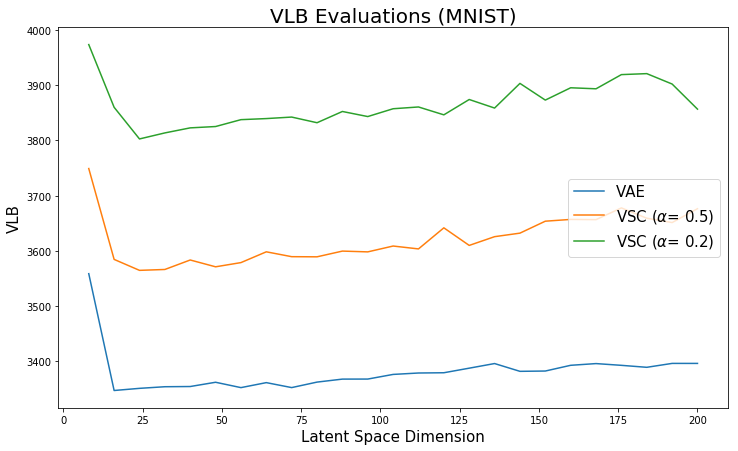
\includegraphics[width=.45\textwidth]{figures/mnist_vlb} &
    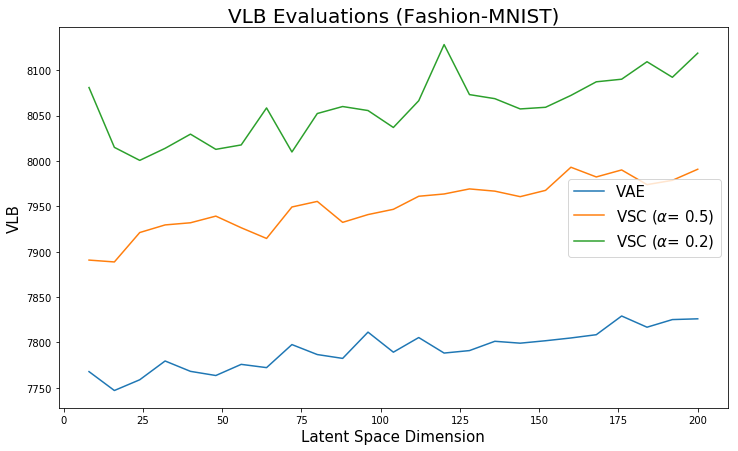
\includegraphics[width=.45\textwidth]{figures/mnist_fashion_vlb} \\
    \textbf{(a)}  & \textbf{(b)}   \\[6pt]
\end{tabular}
    \centering
    \caption{Evaluation of ELBO on the test set for the VSC trained model at varying number of latent dimensions.}
    \label{fig:vlb}
\end{figure}

\subsection{Classification Performance}
We studied the classification accuracy obtained by using the latent representations as input (Figure \ref{fig:classification}), in order to validate the authors' conclusion that the Variational Sparse Coding learned representations improve the classification results and significantly increase robustness with respect to the latent number of dimensions. We can observe that for both MNIST and Fashion-MNIST, after surpassing the optimal latent dimension of the VAE, the representations learned by the VSC are significantly more informative as the latent dimension increases.

\begin{figure}[h]
    \centering
    \captionsetup{justification=centering,margin=1.3cm}
    \begin{tabular}{ccc}
    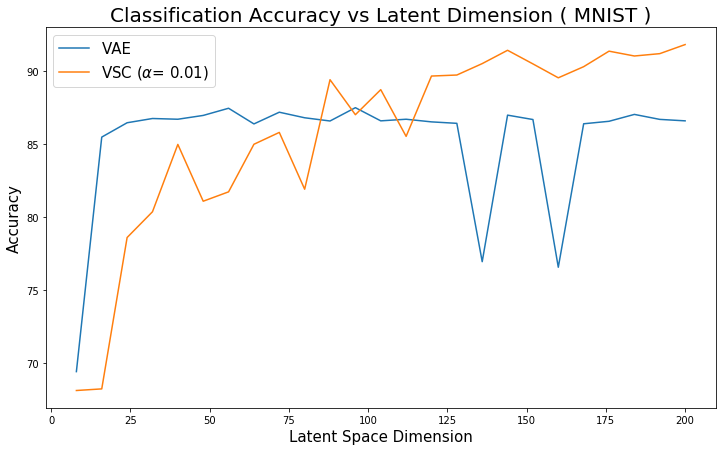
\includegraphics[width=.45\textwidth]{figures/mnist_class} &
    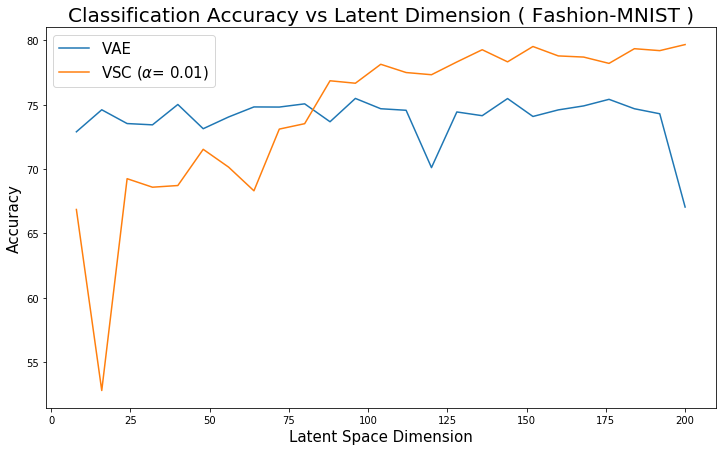
\includegraphics[width=.45\textwidth]{figures/mnist_fashion_class} \\
    \textbf{(a)}  & \textbf{(b)}   \\[6pt]
\end{tabular}
    \centering
    \caption{Classifications results on the test set (for MNIST (a) and Fashion-MNIST (b)) by varying the latent space dimensions using the model VSC - $\alpha = 0.01$ and a 2-layer fully connected neural network as base classifier. }
    \label{fig:classification}
\end{figure}

\subsection{Intepretation of sparse codes}
Authors claim the interpretability of the sparse learned representations. We qualitatively examined the interpretation of the non-zero elements in the sparse codes recovered with the VSC model by running interpolations in the sparse space varying the dimension with the highest absolute value (Figure \ref{fig:reconstruction}). In addition, we observe the effect of the latent dimensionality at capturing the image content (Figure \ref{fig:latent_dim}).

\begin{figure}[!h]
    \centering
    \captionsetup{justification=centering,margin=1cm}
    \begin{tabular}{ccc}
    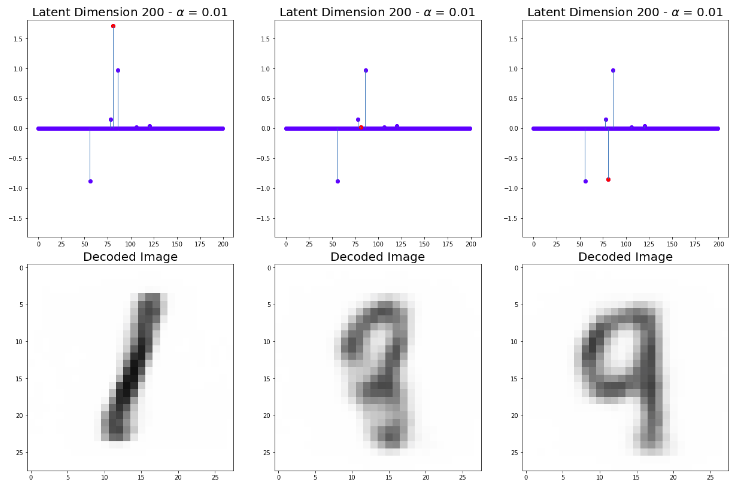
\includegraphics[width=.45\textwidth]{figures/latent200_alpha001_ex2} &
    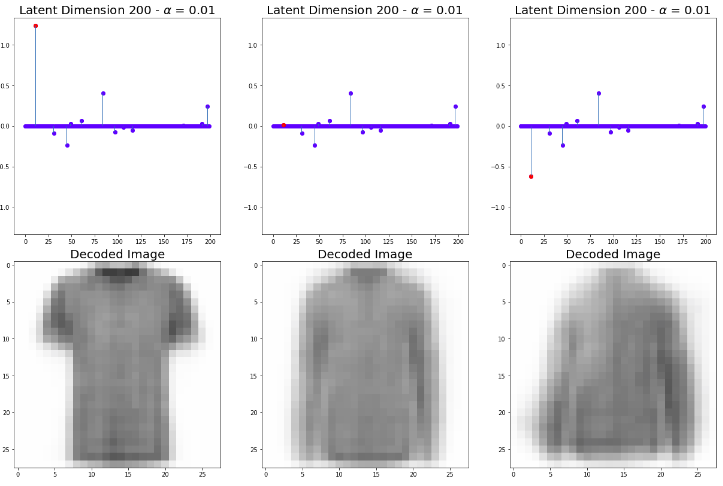
\includegraphics[width=.45\textwidth]{figures/latent200_alpha001_ex4} \\
    \textbf{(a)}  & \textbf{(b)}   \\[6pt]
\end{tabular}
    \centering
    \caption{Reconstruction results by modifying encoding in 200-dimensional latent space for MNIST (a) and Fashion-MNIST (b) for the model VSC - $\alpha = 0.01$.}
    \label{fig:reconstruction}
\end{figure}

\begin{figure}[!h]
    \centering
    \begin{tabular}{ccc}
    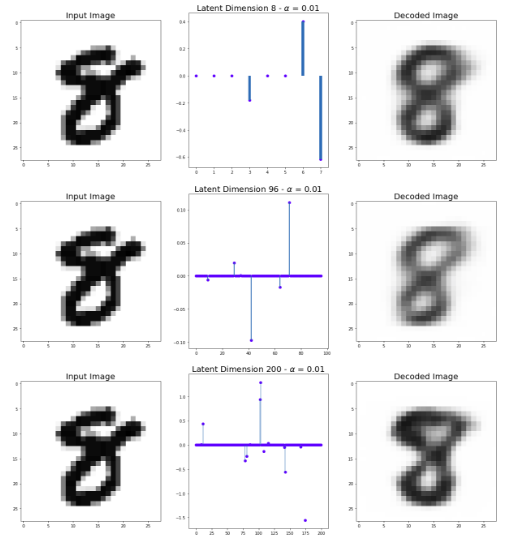
\includegraphics[width=.45\textwidth]{figures/latent_mnist_example} &
    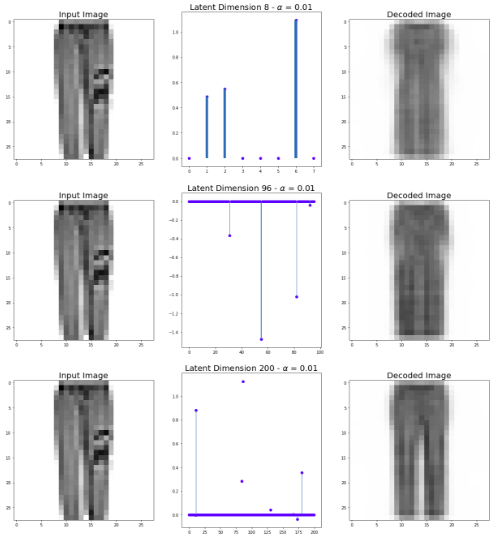
\includegraphics[width=.45\textwidth]{figures/latent_fashion_example} \\
    \textbf{(a)}  & \textbf{(b)}   \\[6pt]
\end{tabular}
    \centering
    \caption{Encoding and reconstruction of samples using the VSC - $\alpha = 0.01$ model from MNIST (a) and Fashion-MNIST (b) datasets with varying latent dimensions of $8$, $96$ and $200$. }
    \label{fig:latent_dim}
\end{figure}

\subsection{Visualization / Traversing Latent Space}
We explored how sampling from the latent space distribution can allow us to obtain interpretable variations in the generated images (Figure \ref{fig:traversals}), and also how conditional sampling produces arguably realistic new samples from the same conceptual entity (Figure \ref{fig:conditional}). The traversal of the latent space is performed varying the latent codes with a high absolute value for a given image, one at a time. We can observe that these latent codes indeed represent interpretable features of the datasets, such as the digits shape in MNIST, the color and shape of the clothes in Fashion-MNIST and the orientation, background color, skin color and hair color in the CelebA results.

\begin{figure}[!h]
    \captionsetup{justification=centering,margin=0.3cm}
    \centering
    \begin{tabular}{ccc}
        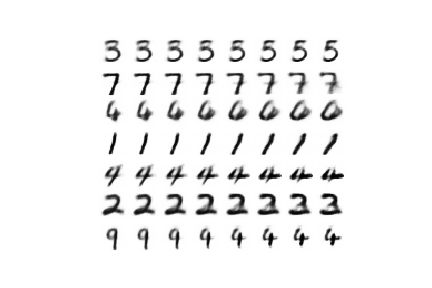
\includegraphics[width=.47\textwidth]{figures/Mnist-traversal} &
        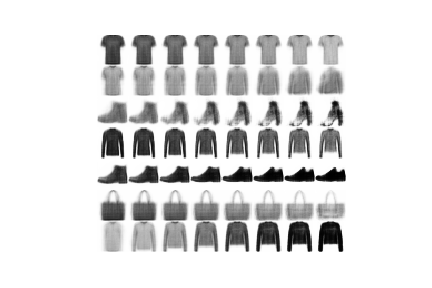
\includegraphics[width=.47\textwidth]{figures/Fashion-traversal} \\
        \textbf{(a)} & \textbf{(b)} \\ [6pt] 
     \end{tabular}
     
     \centering
     \begin{tabular}{cccc}
          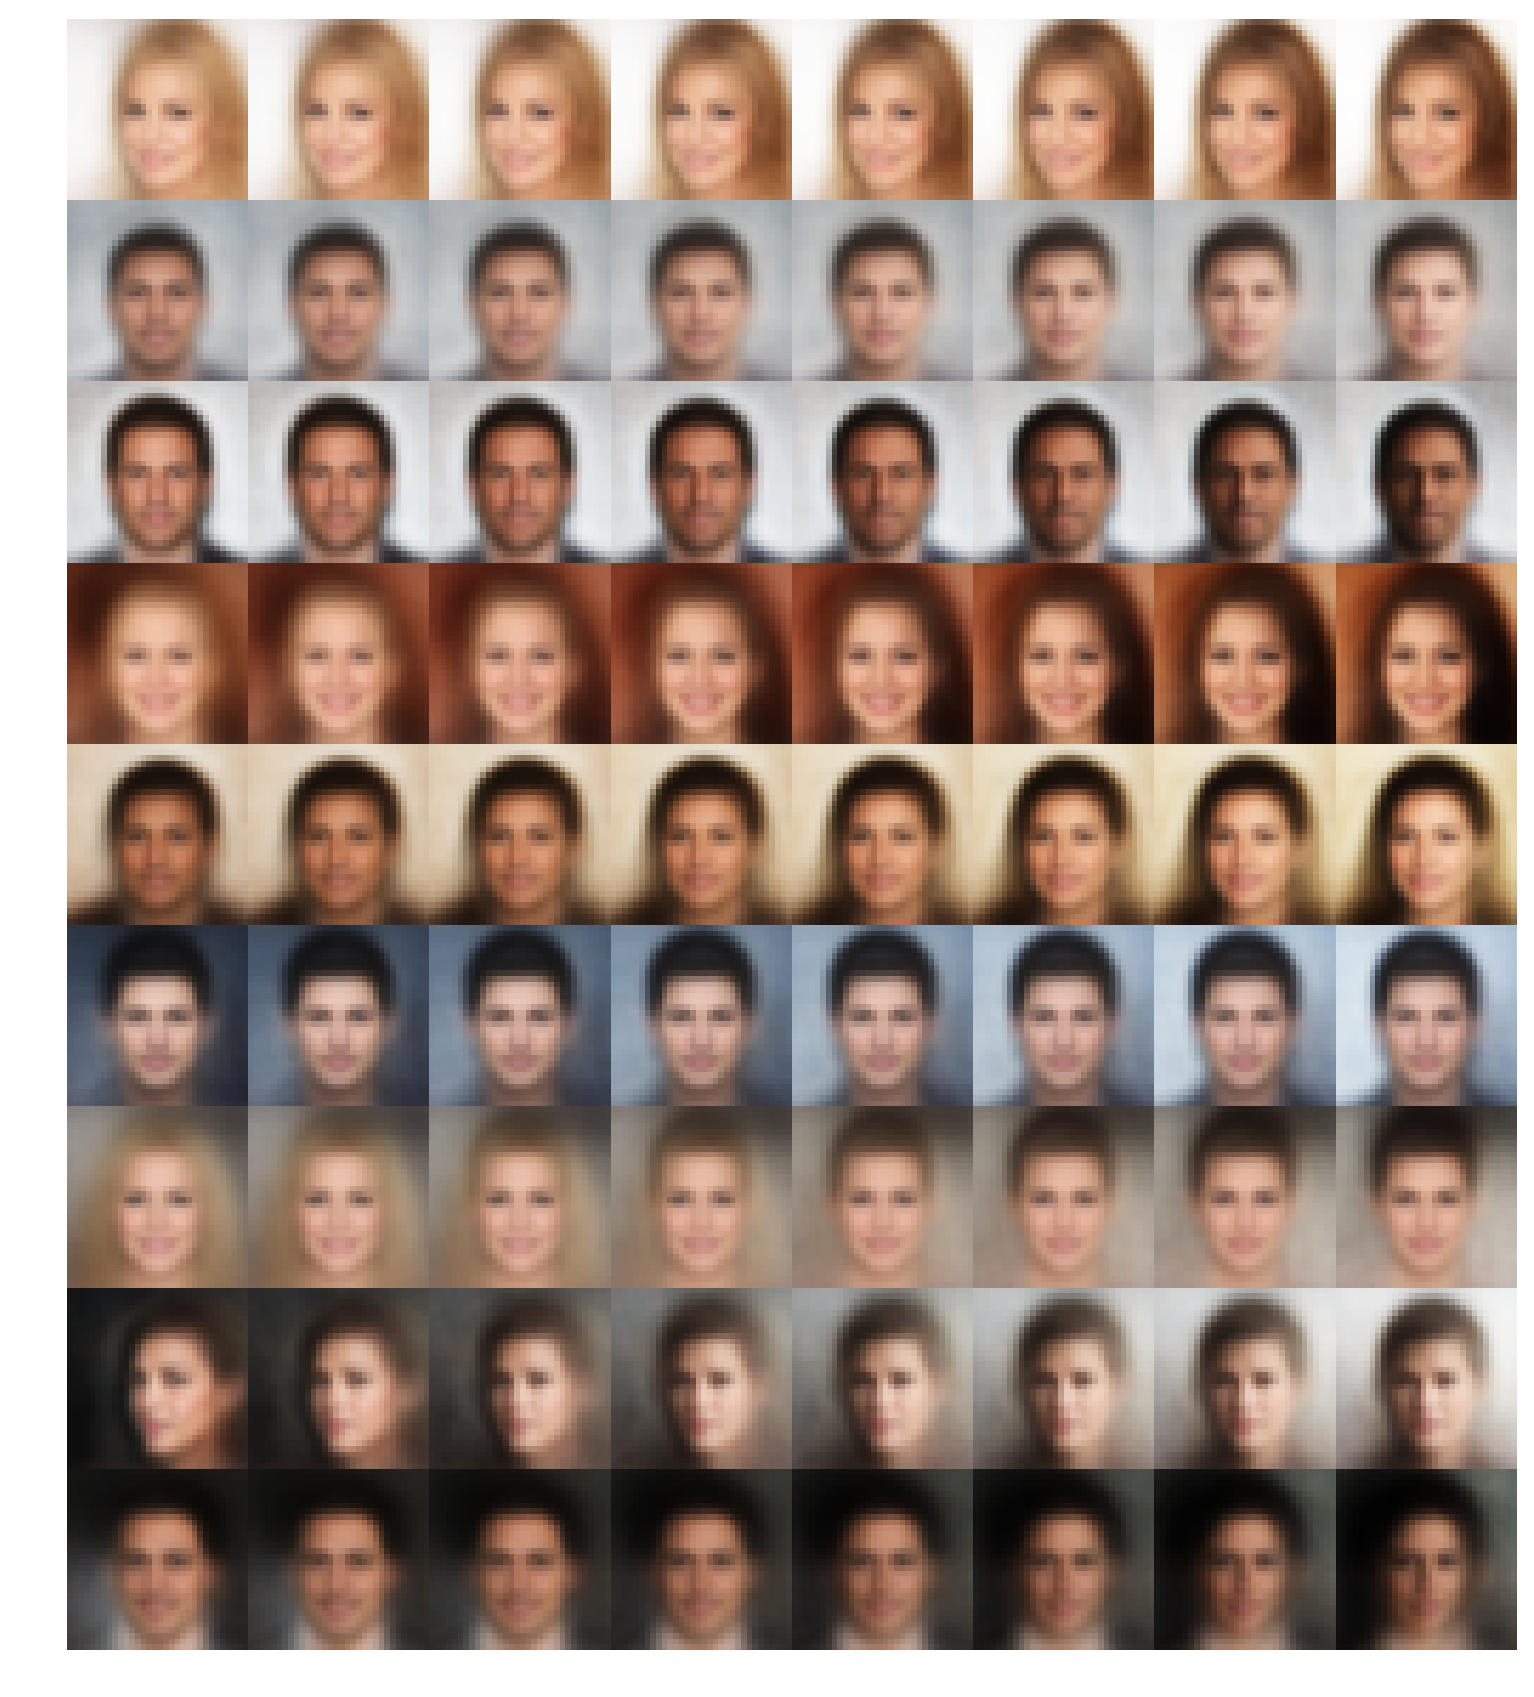
\includegraphics[width=.60\textwidth]{figures/CelebA_Traversal} \\
          \textbf{(c)} \\ [6pt] 
     \end{tabular}
   
    \centering
    \caption{Traversing the latent space of the VSC - $\alpha = 0.01$ model trained for $11$ epochs on MNIST (a) and Fashion-MNIST (b) datasets, and $90$ epochs on CelebA (c) dataset.}
    \label{fig:traversals}
\end{figure}

\begin{figure}[!h]
    \captionsetup{justification=centering,margin=2cm}
    \centering
    \begin{tabular}{ccc}
    
\includegraphics[width=.45\textwidth]{figures/mnist_conditional} &
    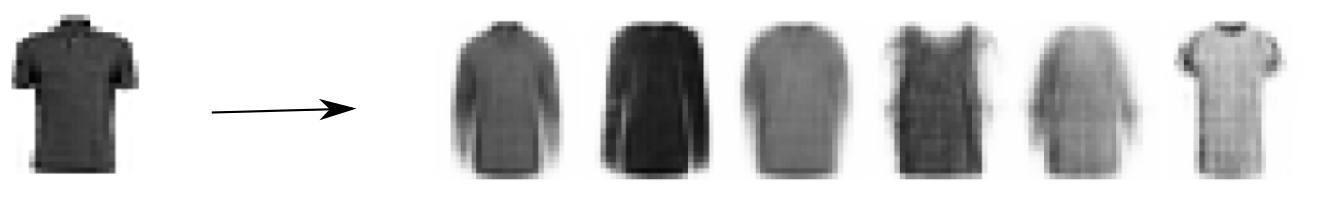
\includegraphics[width=.45\textwidth]{figures/mnist_fashion_conditional} \\
    \textbf{(a)}  & \textbf{(b)}   \\[6pt]
\end{tabular}
    \centering
    \caption{Conditional sampling from VSC - $\alpha = 0.01$ model trained for $11$ epochs on MNIST (a) and Fashion-MNIST (b) datasets.}
    \label{fig:conditional}
\end{figure}


\section{Analysis and discussion of findings}
\label{insights}

We should note that the paper we reproduced was clearly written and overall, despite a few implementation details unspecified (batch size, number of epochs for the CelebA training and weights initialization procedure), it is possible to replicate the results reported. Moreover, we are able to validate the authors hypothesis that the VSC models generate sparse, informative and interpretable representations. \\

Minor discrepancies in the results can be explained by the restricted number of training epochs. In particular, in Figure \ref{fig:vlb}, we observe a similar trend that the one shown in the paper; however, the gap between the curves can be decreased by training the model for larger number of iterations. Furthermore, in the log optimization files, we can easily notice that by using only $20K$ iterations the model has not reached a local optimum yet.  This situation is also present during training on the CelebA dataset: we noticed that at least $50$ epochs are needed to be close to a local optimum, as it is shown in Figure \ref{fig:CelebALoss}. We believe that authors must provide more specifications on the optimization hyperparameters to facilitate the reproducibility task.

\begin{figure}[h]
    \centering
    \captionsetup{justification=centering,margin=1.3cm}
    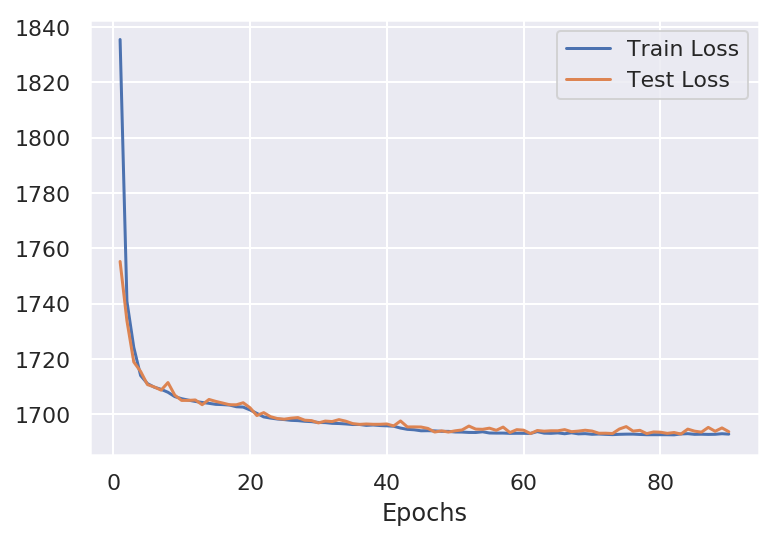
\includegraphics[width=.55\textwidth]{figures/CelebA_Loss}
    \centering
    \caption{Evaluation of training and test loss of the VSC model on the CelebA dataset}
    \label{fig:CelebALoss}
\end{figure}

Similarly, for the classification task (Figure \ref{fig:classification}) although we were able to obtain more informative representations using the VSC model with respect to VAE, the classification accuracy can still be improved by using a higher capacity classification model, instead of the simple classifier used in the original paper. \\

Many of the reviewers addressed the issue of how we can interpret the  learned latent features by the VSC-model. Although authors affirm that the model does not explicitly induce intepretation, it certainly results into a higher expectation of interpretability in large latent spaces, provided that the sources of variations in the observed data can be considered sparse. \\

To account for the blurriness of generated images (Figures \ref{fig:reconstruction} and \ref{fig:traversals}), we must understand that the model capacity is limited and perhaps convolutional architecture could drastically improve the quality of results. 

\section{Conclusions}
\label{conclusions}

% Can we actually validate the results reported? 
Overall the paper describes in enough detail the VSC model implementation and we must applaud the authors in their ability to convey such a complex topic in an approachable and replicable manner. The hypothesis of using Variational Sparse Coding to obtain sparse, informative and interpretable representations was confirmed by reproducing the experiments. \\

% Is it possible to interpret the latent features learned by the VSC model?
Further development on testing the model and comparing it against other sparse models on well known benchmarks is critical. In order to assess how \textit{interpretable} the learned latent features are, we could draw ideas from disentangled representations, to measure the effect of sparsity in the disentanglement metric, against benchmark models such as $\beta$-VAE or Factor-VAE. \\

% How the proposed model can be further improved?
To conclude our reproducibility report we propose the following directions for future research and improvement of current results:
\begin{itemize}
    \item  Increase the number of iterations suggested for training the models and re-run the experiments using the notebooks in our repository.
    \item  In order to improve the quality of generated images, we suggest to expand the model capacity by either stacking more layers or trying convolutional architectures for the encoder and decoder. 
    \item Apply the model to the Disentanglement testing Sprites dataset, to measure the effect of sparsity on a disentanglement metric.
\end{itemize}


\subsubsection*{Acknowledgments}

We would like to thank to Emilien Dupont for clarifying distinct aspects on variational autoencoders' implementation, and Lukas Mosser for his suggestions on training generative models.


% Three years, we launched ReScience, a new scientific journal aimed at publishing the
% replication of existing computational research. Since ReScience published its first
% article\supercite{Topalidou:2015}, things have been
% going steadily. We are still alive, independent and without a budget. In the
% meantime, we have published around 24 articles (mostly in computational
% neuroscience \& computational ecology) and the initial
% \href{https://rescience-c.github.io/board/}{editorial board} has grown from
% around 10 to roughly 100 members (editors and reviewers), we have advertised
% ReScience at several conferences worldwide, gave some
% interviews\supercite{Science:2018}, and published an article introducing
% ReScience in PeerJ~CS\supercite{Rougier:2017}. Based on our
% experience\supercite{Rougier:2018} at managing the journal during these three
% years, we think that time is ripe for some changes.

% \subsubsection{ReScience C \& ReScience X}

% The biggest and most visible change we would like to propose is to change the
% name of the journal ``ReScience'' in favor of ``ReScience C'' where the C
% stands for (c)omputational. This change would be necessary to have consistent
% naming with the upcoming creation of the ``ReScience X'' journal that will be
% dedicated to e(x)perimental replications and co-directed by E.Roesch
% (University of Reading) and N.Rougier (University of Bordeaux). The name
% ``ReScience'' would then be used for the name of a non-profit organization
% (that is yet to be created) for the two journals as well as future journals
% (such as the utopian CoScience\supercite{Rougier:2017} or a future and
% tentative ``ReScience T'' for theoretical science).


% \subsubsection{A new submission process}

% The current submission process requires authors to fork, clone and branch the
% submission repository in order to write their article and to place code and
% data at the relevant places in the forked repository. Once done, authors have
% to push their changes and to make a pull request that is considered as a
% submission. This process is cumbersome for authors and has induced many
% troubles for editors as well once the article is accepted and ready to be
% published, mostly because of the complexity of the editing procedure. In order
% to make life easier for everyone, we greatly simplified the submission process
% for ReScience C and X. Authors are now responsible for getting a DOI for their
% code \& data and only have to submit a PDF and a metadata file in a GitHub
% issue.
% We also provide Python programs that largely automate the subsequent editing
% process. We will still archive the submission on Zenodo but this archive will
% be made for the final PDF only. However, both the PDF and the Zenodo entry will
% contain all associated DOIs (data and code).


% \subsubsection{A simplified publishing process}

% In ReScience, we have have been using a combination of
% \href{https://daringfireball.net/projects/markdown/syntax}{markdown} and
% \href{http://pandoc.org/}{pandoc} for producing both the draft and the final
% version of all the published articles. This had worked reasonably well until it
% started to cause all kind of problems for both authors and editors, especially
% with the reference and citation plugins. Consequently, articles will be now
% submitted directly in PDF with accompanying metadata in a separate file using
% the \href{https://en.wikipedia.org/wiki/YAML}{YAML} format (they were
% previously embedded in the markdown file). Once an article has been accepted,
% authors will be responsible for updating the metadata and for rebuilding the PDF if
% necessary. We could also consider using the
% \href{https://github.com/openjournals/whedon}{Whedon} API that helps with automating
% most of the editorial tasks for \href{http://joss.theoj.org/}{JOSS} and
% \href{http://jose.theoj.org/}{JOSE}. This will most probably require some
% tweaking because our publishing pipeline is a bit different.


% \subsubsection{A new design}

% The combination of markdown and pandoc has also severely limited the layout and
% style possibilities for the article template and since we are switching to
% \LaTeX, this is the opportunity to propose a new design based on a more elegant
% style, using a new font stack\supercite{SourceSerifPro:2014, Roboto:2011,
%   SourceCodePro:2012} (you are currently reading it). The goal is to have a
% subtle but strong identity with enhanced readability. Considering that articles
% will be mostly read on screen (as opposed to printed), we can benefit from a
% more ethereal style. Once this design will have stabilized, an
% \href{https://www.overleaf.com/}{overleaf} template will be made available for
% those without a \TeX~installation. If a \TeX~expert is ready to help review
% the template (and possibly rewrite it as a class), their help would be much
% welcome and appreciated. The same holds for LibreOffice, Word or Pages, any
% template is welcome, just contact us beforehand such that we can coordinate
% efforts.


% \subsubsection{Editorials, letters and special issues}

% ReScience C remains dedicated to the publication of computational replications
% but we (i.e., the editorial team) would like to have the opportunity to
% publish \emph{editorials} when deemed necessary and to give anyone the
% opportunity to write \emph{letters} to the community on a specific topic
% related to reproducibility. Both editorials and letters are expected to be 1 or
% 2 pages long (but no hard limit will be enforced), will be (quickly) peer reviewed,
% and will be assigned a DOI. Furthermore, with the advent of reproducibility
% hackatons worldwide, we will host {\em special issues} with guest editors (such
% as, for example, the organizers of a hackaton) in order to publish the results
% and to enhance their discoverability. Each entry will have to go through the
% regular open peer-reviewed pipeline.\\


% We hope that most readers will agree on the proposed changes such that we can
% commit to them in the next few weeks. The review for this editorial is open (as
% usual) and anyone can comment on and/or oppose any of the proposed changes. New
% ideas are also welcome.
